%%%%%%%%%%%%%%%
\task{Числа и суммы}
\begin{itemize}
\itA Может ли число быть меньше количества цифр в нем? Может ли число быть меньше собственной суммы цифр?

\itB Как по натуральному числу $n$ найти число, не превосходящее его, с наибольшей суммой цифр?

\itC Петя сложил все числа от 1 до $m \cdot n$, а Вася сложил все числа от 1 до $m$, от 1 до $n$ и посчитал произведение этих двух сумм. У кого в итоге получилось большее число?
\end{itemize}
%%%%%%%%%%%%%%%

%%%%%%%%%%%%%%%
\task{Детский сад}
\begin{itemize}
\itA В детском саду 10 детей рисуют 10 рисунков за 20 минут. Как долго 50 детей будут рисовать 50 рисунков? Как долго $d$ детей будут рисовать $r$ рисунков?

\itB Детсадовцам Вове и Диме выдали по обручу — обруч представляет собой диск радиусом $r_1$, из которого вырезан круг радиуса $r_2$, $r_2<r_1$. Мальчики стали клеить пластлин на выданные им обручи. За минуту Вова наращивал сантиметр пластилина на внешнем краю обруча, а Дима — сантиметр пластилина на внутреннем его краю. У кого из мальчиков площадь обруча росла быстрее?

\itC В медпункт детского сада пришло четверо детей. У медсестры есть двухчашечные весы без гирь, и она хочет отсортировать детей по массе. Сколько взвешиваний ей для этого нужно сделать? Как ей производить взвешивания?
\end{itemize}
%%%%%%%%%%%%%%%

%%%%%%%%%%%%%%%
\task{Факториалы}
Факториалом числа $n$ будем называть произведение всех натуральных чисел от 1 до $n$.

\begin{itemize}
\itA Егор посчитал факториал числа 33 и записал его на бумажку. Его сестра решила пошалить, и стерла одну из цифр факториала. Получилась запись:
	$$33! = 8`683`317`618`811`886`49\square`518`194`401`280`000`000$$
Помогите Егору восстановить стертую цифру.

\itB Посчитан факториал числа, не меньшего 12, и из его записи стерта ровно одна цифра — причем известно, с какой позиции. Докажите, что ее всегда можно однозначно восстановить.

\itC Докажите, что при четном $n$ из произведения $1! \cdot 2! \cdot 3! \cdot \ldots \cdot n!$ можно вычеркнуть один факториал так, что оставшееся произведение будет квадратом целого числа.
\end{itemize}
%%%%%%%%%%%%%%%

%%%%%%%%%%%%%%%
\task{В поисках чисел}
\begin{itemize}
\itA Составляя условия олимпиады «Математика НОН-СТОП», мальчики Боря и Дима придумывают для участников математические ребусы: выражения, где разным буквам соответствуют разные цифры. Будут ли ребусы
\begin{center}
	Р$\cdot$О$\cdot$М$\cdot$А$\cdot$Ш$\cdot$К$\cdot$А $=$ РОМАШКА\\
	и \\
	Я$\cdot$О$\cdot$Т$\cdot$Л$\cdot$И$\cdot$Ч$\cdot$Н$\cdot$И$\cdot$К $=$ УРАУРА
\end{center}
иметь решение?

\itB Вася разбил числа от 3 до 8 включительно на четыре группы. Может ли его друг Рома наверняка утверждать, что произведение чисел в одной из этих групп больше 12?

\itC Для данного числа $n$ предъявите алгоритм нахождения наименьшего составного числа $N$ такого, что $n!$ не делится на $N$, и докажите, что полученное составное число действительно будет наименьшим.
\end{itemize}
%%%%%%%%%%%%%%%

%%%%%%%%%%%%%%%
\task{Проблемы завуча}
\begin{itemize}
\itA На параллели 60 школьников ростом 161, 162, ..., 219, 220 сантиметров. Завуч хочет распределить их на три класса так, чтобы минимальный средний рост школьников в классе был максимален. Как ей это сделать?

\itB Завуч, одновременно являясь преподавателем физики, демонстрирует детям абсолютно гибкий, но нерастяжимый и неповреждаемый металлический лист с вырезанным в нем круглым отверстием радиуса $r$. Монета какого максимального диаметра пролезет через это отверстие?

\itC Теперь у завуча есть лист совершенно не гибкого стекла, также с вырезанным в нем круглым отверстием радиуса $r$. Какую длину должно иметь ребро очень шершавого куба, чтобы он не пролезал через это отверстие?
\end{itemize}
%%%%%%%%%%%%%%%

%%%%%%%%%%%%%%%
\task{Фигуры в шахматах}
\begin{itemize}
\itA Какое минимальное количество клеток нужно пройти ферзю из\linebreak точки $(a,b)$ в точку $(c,d)$ на шахматном поле?

\itB Фигура Корблюд умеет делать из данной клетки на шахматном поле четыре хода так, как показано на рисунке 3. Доказать, что корблюд может прийти из любой клетки бесконечного шахматного поля в любую другую. А верно ли такое утверждение для Корблюда Диагонального, делающего ходы как на рисунке 4?

\itC Будем рассматривать фигуры, которые из данной клетки умеют делать четыре хода: вперед-налево, вперед-направо, назад-налево, назад-направо. При этом направо / налево фигура смещается лишь на одну клетку, а вперед / назад каждый ход — либо на две, либо на три клетки. Сколько фигур, с точностью до симметрий, удовлетворяют этим свойствам, и какие из них могут из любой клетки бесконечного шахматного поля дойти до любой другой?
\end{itemize}

\begin{center}
  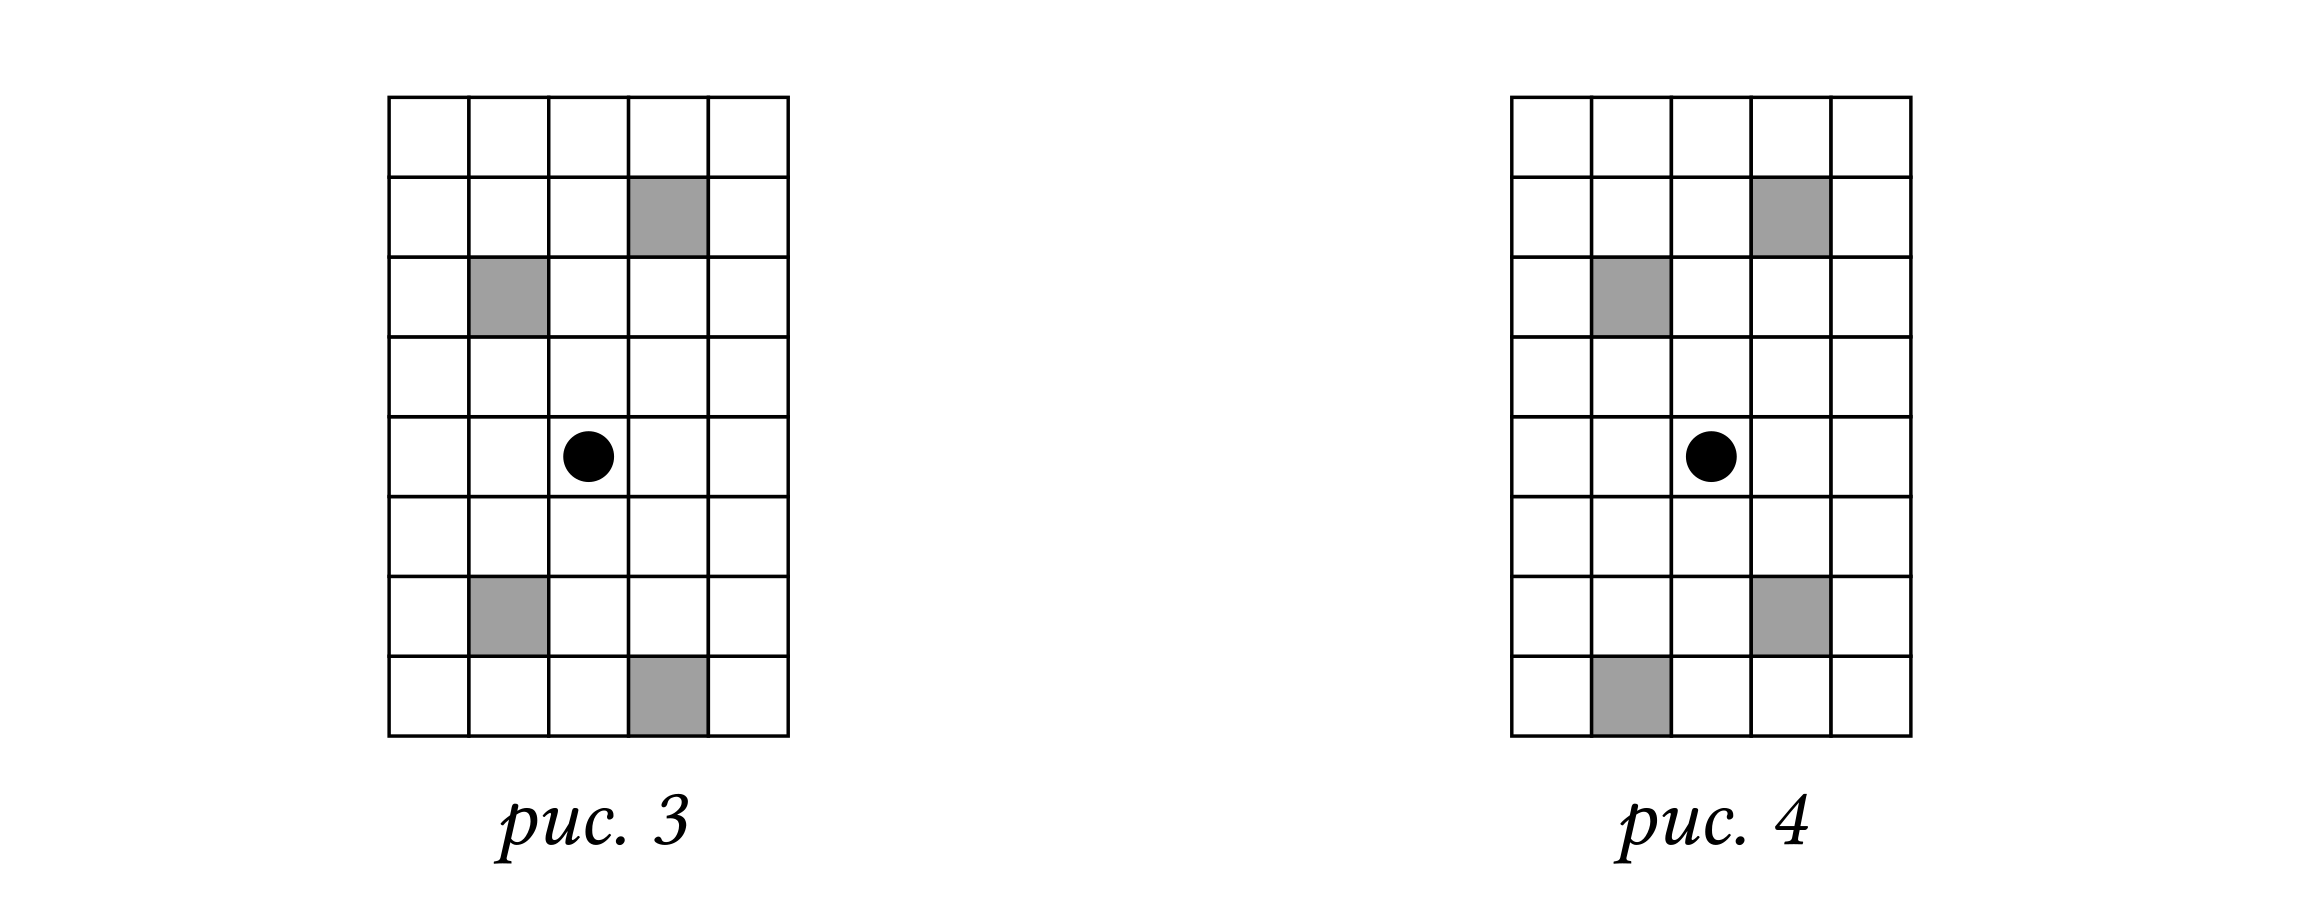
\includegraphics[width=8.5cm]{stats/2016/Figures/Corbleud.png}
\end{center}
%%%%%%%%%%%%%%%

%%%%%%%%%%%%%%%
\task{Пятница}
\begin{itemize}
\itA По пятницам мама наливает пятерым детям парного коровьего молока. Она делает это в два круга, в первый раз как-то наполняя пять кружек, а во второй раз расходуя горшок до конца так, что уровень молока во всех кружках становится одинаковым. После первого\linebreak круга в кружках четырех детей было одинаковое количество молока, а в кружке пятого было на 20\% больше этого количества. Сколько миллилитров составляла эта самая двадцатипроцентная разница, если горшок имеет объем 2 литра, а на втором круге мама использовала 70\% его объема?

\itB По пятницам в селе Хотчланд устраивались бега быков, но в качестве быков использовались тигры. У каждого тигра на ошейнике написаны два числа: $q$ — во сколько раз этот тигр бегает быстрее человека и $t$ — время в секундах, в течение которого этот тигр бежит с максимальной скоростью, а после этого ложится отдохнуть. Помогите участнику бегов Исинбаю Еленову вывести формулу для расстояния $x$, на котором ему нужно держаться от данного тигра, чтобы не быть съеденным.

\itC У мальчика Дани пять пятниц на неделе, а у Кости — три пятницы на неделе. Сколько существует расстановок пятниц на неделе таких, что ровно два дня будут пятницей и для Дани, и для Кости?
\end{itemize}
%%%%%%%%%%%%%%%

%%%%%%%%%%%%%%%
\task{Очень умные муравьи}
\begin{itemize}
\itA На плоскости живут четыре муравья. Могут ли они нарисовать себе на плоскости четыре связные области так, чтобы любые два муравья могли бы общаться друг с другом~— их области имели бы участок общей границы?

\itB Человек соорудил муравьям планету, то есть подвесил в воздух коробку размером $1 \times 1 \times 1$ метр. Через некоторое время он заметил, что муравьи организовывают экспедиции к углам коробки, как будто ходят в горы. Рост муравья — 2мм. Подъему на холм какой высоты для человека нормального роста соответствует восхождение муравья к углу коробки, если рост нормального человека равен двум метрам?

\itC Счетное сообщество муравьев хочет организовать на плоскости\linebreak треугольную сетку такую, чтобы к каждой вершине прилегало ровно пять треугольников, жители которых могли бы попить чай в этой вершине. По силам ли муравьям это предприятие?
\end{itemize}
%%%%%%%%%%%%%%%

%%%%%%%%%%%%%%%
\task{Эксперименты с клавиатурой}
\begin{itemize}
\itA У братьев А. и Б. на клавиатурах начался {\itshape дребезг}: у А. все сим-\linebreak волы набирались пятикратно, а {\verb!Backspace!} удалял сразу восемь последних напечатанных символов. У Б. символы набирались семь раз подряд, а {\verb!Backspace!} удалял последние четыре напечатанных символа. При равной скорости нажатия на клавиши, кто из братьев будет печатать быстрее?

\itB Починив дребезг, братья обнаружили другие неполадки: у А. сломалась клавиша {\verb!Shift!}, а у Б. — {\verb!Caps Lock!}. До поломки оба печатали с одинаковой скоростью: они нажимали по пять клавиш в секунду. Неисправности повлияли на скорость печати: теперь А. должен нажимать {\verb!Caps Lock!} перед каждой последовательностью заглавных букв и еще раз нажимать после нее, а Б. — удерживать {\verb!Shift!}, чтобы печатать заглавные буквы: при этом его скорость падает до двух букв в секунду, но на нажатие {\verb!Shift!} время не тратится. Вам нужно придумать строчку, которую А. напечатает минимум в два раза быстрее, чем Б. А есть ли строчка, которую Б. печатает в два раза быстрее, чем А.?

\itC Через год у Б. на клавиатуре осталось две рабочих клавиши, да и печатать он стал медленнее: нажимает лишь четыре клавиши в секунду. Паузы в процессе набора информации не несут;  две клавиши одновременно нажимать нельзя. Вам нужно придумать способ без уменьшения русского алфавита (признания каких-нибудь букв равными) набирать любую букву не более чем за секунду либо доказать, что такого способа нет. Если его нет, то какое минимальное количество букв достаточно отождествить в одну, чтобы он появился?
\end{itemize}
%%%%%%%%%%%%%%%

%%%%%%%%%%%%%%%
\task{Первым делом — самолеты}
\begin{itemize}
\itA Комната освещена маленькой лампой, установленной на стене. Петя пускает бумажные самолетики так, что они пролетают перед\linebreak лампочкой на ее уровне. Вася же берется определить, был пролетающий самолетик наклонен к лампочке или от лампочки, лишь по длине теней от его крыльев на противоположной стене. Как ему это сделать?

\itB Четыре маленьких вертолета стоят на земле в вершинах квадрата $1 \times 1$ метр. На какую высоту нужно взлететь двум из них, чтобы попарные расстояния между вертолетами стали одинаковыми?

\itC По прямым, содержащим стороны правильного семиугольника со стороной в два километра, перемещаются камеры. Оператору Blue Origin было дано задание посадить ракету в этот семиугольник так, чтобы суммарное расстояние от нее до прямых, по которым ездят камеры, было минимальным. Куда оператору сажать ракету?
\end{itemize}
%%%%%%%%%%%%%%%

%%%%%%%%%%%%%%%
\task{Несправедливый турнир}
\noindent Турнир по скоростному распиливанию проходит по усовершенствованной олимпийской системе. Изначально в турнире $2^t$ участников, $t \geq 2$, все в одной группе, потом группа потихоньку дробится: в каждом раунде в каждой группе участники бьются на пары, в которых состязаются в распиливании, и после раунда образуются группа победителей и группа проигравших, где повторяется аналогичный турнир.

\ms Так продолжается, пока все участники не побьются на группы по одному человеку: тогда места участников в итоговой таблице определяются естественным образом. В частности, победитель турнира — участник, выигравший во всех $t$ раундах, а аутсайдер — проигравший во всех $t$ раундах.

\begin{itemize}
\itA Может ли самый слабый участник турнира не оказаться аутсайдером?

\itB Может ли состязающийся сильнее как минимум половины участников турнира и еще одного человека встретиться в финале с аутсайдером?

\itC Доказать, что для всякого состязающегося слабее половины участников турнира можно подобрать разбиение на пары в раундах так, чтобы в финале он встретился с аутсайдером.
\end{itemize}
%%%%%%%%%%%%%%%

%%%%%%%%%%%%%%%
\task{Попытки осмысления биссектрис}
\begin{itemize}
\itA У Робинзона Крузо есть стандартный советский чертежный треу-\linebreak гольник с углами в 30, 60 и 90 градусов. Как ему с помощью этого треугольника начертить на песке угол в 15 градусов?

\itB Мальчик по имени Текдра решил определять биссектрису трехгранного угла следующим образом: проведем биссектрису одной из его граней, затем плоскость, проходящую через эту биссектрису и противоположное использованной грани ребро. Теперь проведем биссектрису угла в этой плоскости, образованного ребром и старой\linebreak биссектрисой. Докажите, что определение Текдры некорректно — в одном трехгранном угле можно построить несколько различных биссектрис.

\itC В треугольнике $MNK$ проведены биссектрисы углов $N$ и $K$. Из оставшейся вершины на эти биссектрисы опустили перпендикуляры и провели прямую через их основания. Доказать, что она будет параллельна стороне $NK$.
\end{itemize}
%%%%%%%%%%%%%%%